\documentclass[12pt,fleqn]{article}
%\usepackage {psfig,epsfig} % para incluir figuras em PostScript
\usepackage{amsfonts,amsthm,amsopn,amssymb,latexsym}
\usepackage{graphicx}
\usepackage[T1]{fontenc}
\usepackage[brazil]{babel}
\usepackage{geometry}
\usepackage[utf8]{inputenc}
\usepackage[intlimits]{amsmath}
\graphicspath{{./images/}}
%alguns macros
\newcommand{\R}{\ensuremath{\mathbb{R}}}
\newcommand{\Rn}{{\ensuremath{\mathbb{R}}}^{n}}
\newcommand{\Rm}{{\ensuremath{\mathbb{R}}}^{m}}
\newcommand{\Rmn}{{\ensuremath{\mathbb{R}}}^{{m}\times{n}}}
\newcommand{\contcaption}[1]{\vspace*{-0.6\baselineskip}\begin{center}#1\end{center}\vspace*{-0.6\baselineskip}}
%=======================================================================
\usepackage{a4}                       % tamanho da página
\setlength{\textwidth}{16.0cm}        % largura do texto
\setlength{\textheight}{9.0in}        % tamanho do texto (sem head, etc)
\renewcommand{\baselinestretch}{1.15} % espaçamento entre linhas
\addtolength{\topmargin}{-1cm}        % espaço entre o head e a margem
\setlength{\oddsidemargin}{-0.1cm}    % espaço entre o texto e a margem

% Ser indulgente no preenchimento das linhas
\sloppy


\begin{document}


\pagestyle {empty}

% Páginas iniciais
\vspace*{-2cm}
{\bf
\begin{center}
{\large
\hspace*{0cm}Universidade de São Paulo} \\
\hspace*{0cm}Escola Politécnica \\
\hspace*{0cm}Curso de Engenharia de Computação  \\
\end{center}}
\centerline{
\includegraphics[scale=0.8]{logo-poli}}
\vspace{.5cm}
\noindent
\begin{center}
{\Large \bf Condução de calor em placa plana com fontes e sorvedouros} \\[2cm]
{\Large Tiago Koji Castro Shibata (8988730), tiago.shibata@usp.br}\\[6mm]
{\Large Deborah Hidemi Kamiguchi Watanabe (4430967), deborah.watanabe@usp.br}\\[6mm]
\vspace{.5cm}
\end{center}

{\raggedleft
\begin{minipage}[t]{8.0cm}
\setlength{\baselineskip}{0.25in}
RELATÓRIO apresentado ao Professor Alexandre Roma do MAP/IME-USP
como atividade da disciplina MAP3122 - Métodos Numéricos.
\end{minipage}\\[2cm]}

\vspace{1cm}
{\center São Paulo - SP \\[3mm]
31/03/2016 \\}

\newpage


\pagestyle {empty}
\abstract{A geração de calor está presente no dia a dia de todos os seres. Desde as perdas de energias ocorrentes na mais simples das reações biológicas, o calor muitas vezes representa a energia desperdiçada, o movimento caótico de moléculas que se dispersam do fenômeno sendo realizado.

Na engenharia, a geração de calor e principalmente o aumento de temperatura têm grandes consequências, podendo criar um ambiente desagradável em uma construção mal planejada, queimar um motor ou causar danos em equipamentos. Em eletrônica, o aumento de temperatura leva circuitos a queimarem ou desligarem-se se possuírem proteção contra sobretemperatura. Neste trabalho, focamos em um modelo simples de condução de calor, em uma placa plana. A placa possuirá fontes e sorvedouros, simulando a ação de uma placa eletrônica metálica contendo componentes integrados. Algumas regiões (com componentes) serão tradadas como fontes de calor, e a placa como um todo terá uma pequena perda de calor (representando a troca de calor com o ar).

Nesse trabalho, desejamos simular a condução de calor em uma barra ou placa a partir da equação de difusão de calor, aplicando métodos numéricos em soluções computacionais. Obteremos mapas de temperatura e fluxo de calor para diferentes condições e configurações. Apresentando a temperatura próxima aos componentes, podemos simular a temperatura na qual a placa final operará e tentar melhorar a disposição dos mesmos.}

\newpage

\tableofcontents

% Numeração em romanos para páginas iniciais (sumários, listas, etc)
%\pagenumbering {roman}
\pagestyle {plain}

\setcounter{page}{0} \pagenumbering{arabic}

\setlength{\parindent}{0in}  %espaco entre paragrafo e margem
% Espaçamento entre parágrafos
\parskip 5pt
\newpage
\section{Introdução}

%comando cria itens
\begin{itemize}
	\item introduzir o problema a ser estudado
	\item apresentar trabalhos relacionados
	\item apresentar motivação
	\item apresentar objetivos
	\item Último parágrafo deve conter a organização do documento
\end{itemize}

\section{Modelo}
Em nosso modelo, a placa plana será discretizada em múltiplos quadrados de dimensão pequena. Cada pequeno quadrado será a menor subdivisão da placa que trataremos e possuirá uma temperatura homogênea. Essa resolução é baseada nos métodos de elementos finitos, onde uma subdivisão fina e finita de uma peça permite aproximações numéricas de fenômenos em objetos complexos e difíceis de resolver analiticamente. No entanto, em elementos finitos cada elemento é geralmente representado por uma forma não uniforme. Nesse trabalho, os elementos serão uniformes, bidimensionais e retangulares, sempre.

As condições iniciais serão tomadas como temperatura homogênea em toda a placa (placa desligada e equilibrada). O calor gerado pelos componentes será tomado de seus datasheets e seu número e posições será configurável. Utiliza-se o modelo de placa bidimensional, homogênea e isotrópica, ou seja, suas propriedades não se alteram em diferentes direções ou posições e a condução térmica é constante em toda a sua extensão.

O fluxo de energia térmica, que indica locais com grande variação (gradiente) de temperatura, é proporcional ao inverso do gradiente da temperatura (os operandos de u(x, y, t) foram omitidos por simplicidade) \cite{ufsc_geracao_de_calor}:

\[q = -k A \Delta u\]


\section{Exemplos de Equações}
Nesta seção serão apresentados diferentes exemplos de equações.

\subsection{Equações simples}

\textbf{Sem numeração}
\[\sum_{i=1}^{100}\frac{2^{i-1}}{4}\]

\textbf{Com numeração}
\begin{equation}
	\int_{0}^{100}\sqrt[4]{\frac{2n}{7}}
\end{equation}

\begin{equation}
M^{-1}(AD^{-1}A^T)M^{-T}\bar{y} = M^{-1}(AD^{-1}(r_d -X^{-1}r_a) + r_p),
\end{equation}


\subsection{Equações com mais de uma linha}
\begin{eqnarray}
\label{pp} %faz um r�tulo na equa��o. Ser� usado para referenci�-la.
\min & c^Tx \\ \nonumber
\mbox{s.a.} & Ax=b \\ \nonumber
            & x \geq 0, \nonumber
\end{eqnarray}
onde $A \in \Rmn$, $b \in \Rm$ and $c \in \Rn$.
Referenciando a equação ~(\ref{pp})

\subsection{Sistema linear}

\begin{equation}
 \left[
\begin{array}{ccc}
 A & 0   & 0 \\
 0 & A^T & I\\
 Z & 0   & X
\end{array} \right]
\left[
\begin{array}{c}
 x \\
 y \\
 z \\
\end{array}
\right]
=
\left[
\begin{array}{c}
 1 \\
 2 \\
 3
\end{array}
\right]
\label{eqpc0}
\end{equation}

\[
d_i=\left \{
\begin{array}{cc}
1 & \mbox{se } i=0 \\
2 & \mbox{caso contrário}\\
\end{array}
\right \}
\]

%inicia uma nova p�gina
\clearpage

\section{Tabelas}
\label{sec:tab}


\subsection{Tabela Simples}
\begin{table}[htb]
\begin{center}
		\begin{tabular}{|c|c|c|}\hline
		12  & 13 & 14 \\\hline
		15  & 16 & 17 \\\hline
		\end{tabular}
\label{tab:Tabela1}
\caption{Título da tabela}
\end{center}
\end{table}


\subsection{Tabela mais elaborada}
\begin{table}[htb]
\begin{center}
\begin{tabular}{|l|r|c|r|r|} \hline
            & \multicolumn{2}{|c|}{{CCF preconditioner}} & \multicolumn{2}{|c|}{{Number of nonzeros}} \\ \cline{2-5}
{Problem}   & \multicolumn{1}{|c|}{$\eta$}  & \multicolumn{1}{|c|}{$ \frac{n(AD^{-1}A^T)}{nrow}$} & \multicolumn{1}{|c|}{FCC} & \multicolumn{1}{|c|}{Cholesky}  \\ \hline \hline
ELS-19    &  -11 & 31 &  87750  & 3763686  \\\hline
SCR20     &  -12 & 31 &  103179 & 2591752  \\\hline
NUG15     &  -12 & 32 &  54786  & 6350444 \\\hline
PDS-20    &   15 & 5  &  625519 & 7123636\\\hline
\end{tabular}
\caption{Título da Tabela.}
\label{tabn}
\end{center}
\end{table}

Referenciando a tabela~\ref{tabn}.

\section{Edição}

Comando para preservar a formatação do texto.
\begin{verbatim}
#include <iostream>         // < > is used for standard libraries.
void main(void)             // ''main'' method always called first.
{
 cout << ''This is a message.'';
                            // Send to output stream.
}
\end{verbatim}

\section{Inserir figuras}

\begin{figure}[htb]
	\centering
		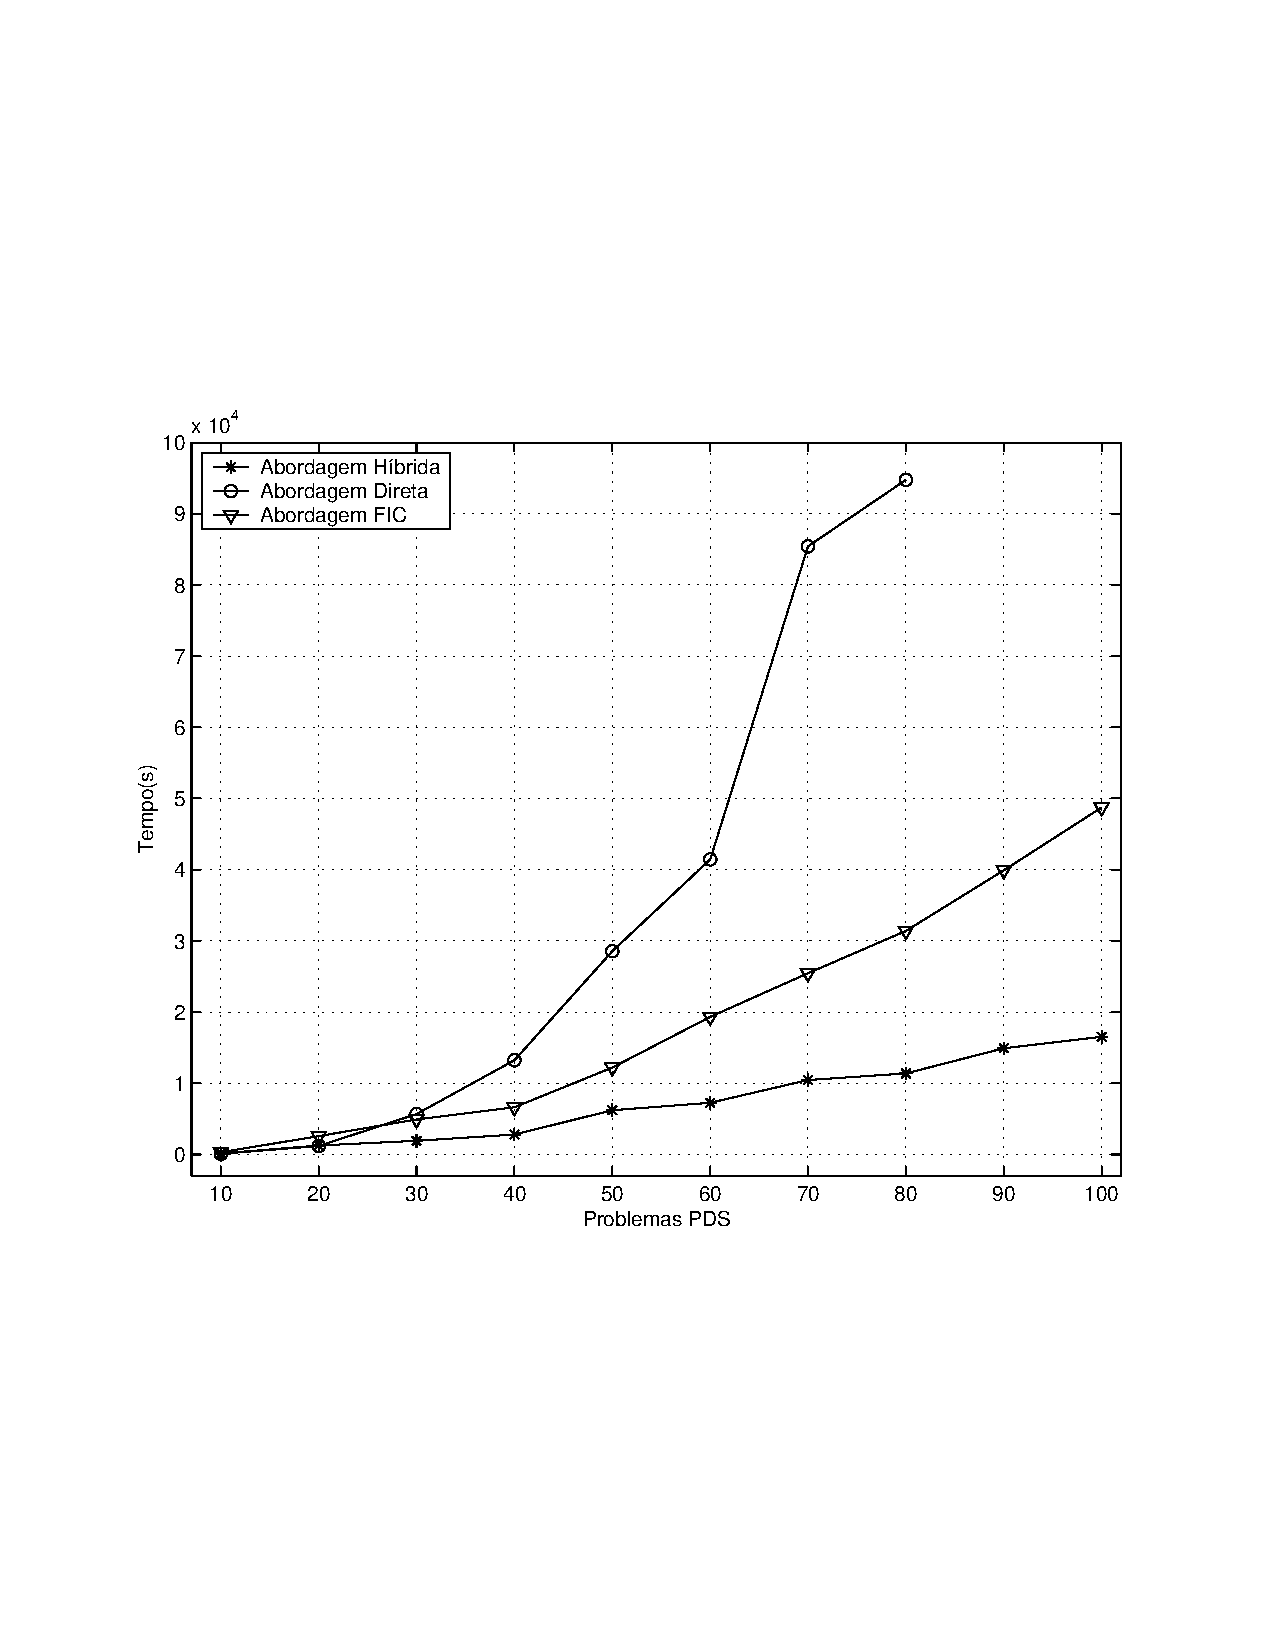
\includegraphics[height=14cm]{figura}
	\label{fig:pdsmodel}
\end{figure}

%\clearpage %come�a nova p�gina

Para citar referências bibliográficas~\cite{Adler89}, \cite{Carmo05}.

\section{Conclusões}
Apresentar as conclusões finais.

\vspace{5mm}
{\bf{Agradecimentos}} Agradecimentos aos colaboradores, professores que eventualmente procuraram para ajudar em
algum aspecto do modelo, colega que ajudou a compor alguma parte do trabalho e assim por diante.

\bibliographystyle{plain}
\bibliography{bibliografia}

% aqui, viriam os ap�ndices se viessem (fica como atividade descobrir como introduz�-los

\end{document} %finaliza o documento
